\section{PDE1: Advection-Diffusion Equation with Spatially Distributed Velocity Field}
\label{sec:AD}

\renewcommand{\thefigure}{C.\arabic{figure}}  % Number figures as A.1, A.2, ...
\renewcommand{\thetable}{C.\arabic{table}}  % Number tables as A.1, A.2, ...


\subsection*{Problem setup}
We model the transport of a concentration field \( C(\textbf{x}, t) \) in a two-dimensional spatial domain \(\mathcal{X} = [0, 1.0] \times [0, 1.0]\) over time \( t \in [0, 1.0] \), governed by the advection-diffusion equation with a spatially varying velocity field. Defining \( \textbf{x} = (x_1, x_2) \in \mathcal{X} \), the system is:
\begin{equation}
\frac{\partial C}{\partial t} + \nabla \cdot \bigl( \mathbf{u}(\textbf{x}) C \bigr) = D \nabla^2 C,
\label{eq:advection-diffusion}
\end{equation}
where \( C(\textbf{x}, t) \) is the concentration, \(\mathbf{u}(\textbf{x}) = [u_x(\textbf{x}), u_y(\textbf{x})] \) is the velocity field with components \( u_x(\textbf{x}) = u_x(x_1, x_2) \) and \( u_y(x) = u_y(x_1, x_2) \), and \( D = 0.005 \) is the constant diffusion coefficient. Periodic boundary conditions are applied in both \( x_1 \) and \( x_2 \) directions. The initial condition \( C_0(\mathbf{x}) = C(\mathbf{x}, 0) \) and velocity components \( u_x(\mathbf{x}) \) and \( u_y(\mathbf{x}) \) are sampled from Gaussian random fields (GRFs) with specified parameter ranges:

\begin{equation}
C_0(\mathbf{x}) \sim \text{GRF}(p_{\min} = -1.0, p_{\max} = 2.0, \sigma = 2, \mathcal{X}),
\end{equation}

\begin{equation}
u_x(\mathbf{x}), u_y(\mathbf{x}) \sim \text{GRF}(p_{\min} = -1.0, p_{\max} = 1.0, \sigma = 2, \mathcal{X}).
\end{equation}

\subsection*{Numerical Solver for the Advection-Diffusion Equation}

To generate training data for neural operator learning, we implemented a differentiable numerical solver for the advection-diffusion equation using \texttt{torchdiffeq}, reformulating the system as an ordinary differential equation (ODE):
\begin{equation}
\frac{dU}{dt} = \text{RHS}(\mathbf{x}, t, p),
\end{equation}
where \( U = [C] \) denotes the concentration field, and \( \text{RHS}(\mathbf{x}, t, p) \) encapsulates the advection \( \nabla \cdot (\mathbf{u}C) \) and diffusion \( \nabla^2 C \) terms with \( p = \mathbf{u} = [u_x, u_y] \) as the velocity field. Spatial discretization employs a finite difference method (FDM) on a \( 150 \times 150 \) grid within \( \mathcal{X} \), downsampled to \( S_x = S_y = 50 \) divisions, using a second-order central difference scheme for the Laplacian and an upwind scheme for the advection term to ensure stability. Periodic boundary conditions are enforced via ghost cells to maintain flux continuity. Time integration leverages an explicit fourth-order Runge–Kutta (RK4) scheme with a step size of \( 10^{-4} \), recording solutions at \( t = 0.01 \) intervals over \( [0, T = 1] \), yielding \( n_t = 100 \) time steps. Implemented with gradient tracking in \texttt{torchdiffeq}, the solver computes the Jacobian \( \frac{\partial U}{\partial p} \) with respect to the velocity parameters, supporting sensitivity-aware training in the SC-NO framework.




\subsection*{Neural Operator Learning for the Advection-Diffusion Equation}

We apply neural operator learning to the advection-diffusion equation defined over a spatial domain \( \mathcal{X} = [0, S_x] \times [0, S_y] \subset \mathbb{R}^2 \) with \( \mathbf{x} = (x_1, x_2) \in \mathcal{X} \) and time \( t \in [0, T=1.0] \), discretized into \( n_t \) time steps. The spatially varying velocity field \( \mathbf{u}(\mathbf{x}) = [u_x(\mathbf{x}), u_y(\mathbf{x})] \) serves as the parameter \( p(\mathbf{x}) \) within the input function \( a(\mathbf{x}, t, p) \in \mathcal{U} \), which also includes the first \( t_u \) time steps of the solution \( u(\mathbf{x}, t, p) \). We train a neural operator \( \mathcal{G}_\theta \) in the SC-NO framework to predict the subsequent \( t_G = n_t - t_u \) time steps, guided by the Jacobian \( \frac{\partial u}{\partial p} \), using the mapping:
\begin{equation}
\mathcal{G}_\theta: \left( \mathcal{X} \times [0, t_u], p(\mathbf{x}) \right) \to u(\mathbf{x}, t, p), \quad \text{for } (\mathbf{x}, t) \in \mathcal{X} \times [t_u, T].
\end{equation}
This approach unifies the spatial-temporal input and parameter field to learn a solution operator spanning \( [t_u, T] \) across all PDE instances.


\subsection*{Additional results for PDE1}

% Table for performances of models for forward prediction of PDE1 without STD 
\begin{table}[ht!]
\centering
\caption{\scriptsize\textbf{Comparison of Error Metrics Across Models Trained with Different Sample Sizes (Forward)}}
\label{tab:pde1_forward_nostd}
\scriptsize
\setlength{\tabcolsep}{3pt}
\begin{tabular}{lcccccccc}
\hline
\textbf{Model} & \multicolumn{2}{c}{\textbf{1000 Samples}} & \multicolumn{2}{c}{\textbf{500 Samples}} & \multicolumn{2}{c}{\textbf{200 Samples}} & \multicolumn{2}{c}{\textbf{100 Samples}} \\
 & \textbf{Rel. \(L^2\)} & \textbf{MAE} & \textbf{Rel. \(L^2\)} & \textbf{MAE} & \textbf{Rel. \(L^2\)} & \textbf{MAE} & \textbf{Rel. \(L^2\)} & \textbf{MAE} \\
\hline
FNO        & \(5.1 \times 10^{-2}\) & \(5.6 \times 10^{-3}\) & \(1.7 \times 10^{-1}\) & \(1.9 \times 10^{-2}\) & \(8.5 \times 10^{-1}\) & \(9.4 \times 10^{-2}\) & \(1.4 \times 10^{0}\) & \(1.5 \times 10^{-1}\) \\
WNO        & \(6.2 \times 10^{-2}\) & \(6.6 \times 10^{-3}\) & \(2.0 \times 10^{-1}\) & \(2.2 \times 10^{-2}\) & \(9.8 \times 10^{-1}\) & \(1.1 \times 10^{-1}\) & \(1.6 \times 10^{0}\) & \(1.8 \times 10^{-1}\) \\
DeepONet   & \(6.2 \times 10^{-2}\) & \(6.9 \times 10^{-3}\) & \(2.1 \times 10^{-1}\) & \(2.3 \times 10^{-2}\) & \(1.0 \times 10^{0}\) & \(1.1 \times 10^{-1}\) & \(1.7 \times 10^{0}\) & \(1.8 \times 10^{-1}\) \\
SC-FNO     & \(\mathbf{2.6 \times 10^{-2}}\) & \(\mathbf{1.9 \times 10^{-3}}\) & \(\mathbf{5.5 \times 10^{-2}}\) & \(\mathbf{6.2 \times 10^{-3}}\) & \(\mathbf{1.2 \times 10^{-1}}\) & \(\mathbf{1.4 \times 10^{-2}}\) & \(\mathbf{1.8 \times 10^{-1}}\) & \(\mathbf{2.0 \times 10^{-2}}\) \\
SC-WNO     & \(2.8 \times 10^{-2}\) & \(2.1 \times 10^{-3}\) & \(6.0 \times 10^{-2}\) & \(6.9 \times 10^{-3}\) & \(1.4 \times 10^{-1}\) & \(1.5 \times 10^{-2}\) & \(2.0 \times 10^{-1}\) & \(2.2 \times 10^{-2}\) \\
SC-DeepONet& \(3.2 \times 10^{-2}\) & \(2.5 \times 10^{-3}\) & \(7.5 \times 10^{-2}\) & \(8.4 \times 10^{-3}\) & \(1.6 \times 10^{-1}\) & \(1.9 \times 10^{-2}\) & \(2.4 \times 10^{-1}\) & \(2.7 \times 10^{-2}\) \\
\hline
\end{tabular}
\end{table}





% \begin{figure}[ht!]
%     \centering
%     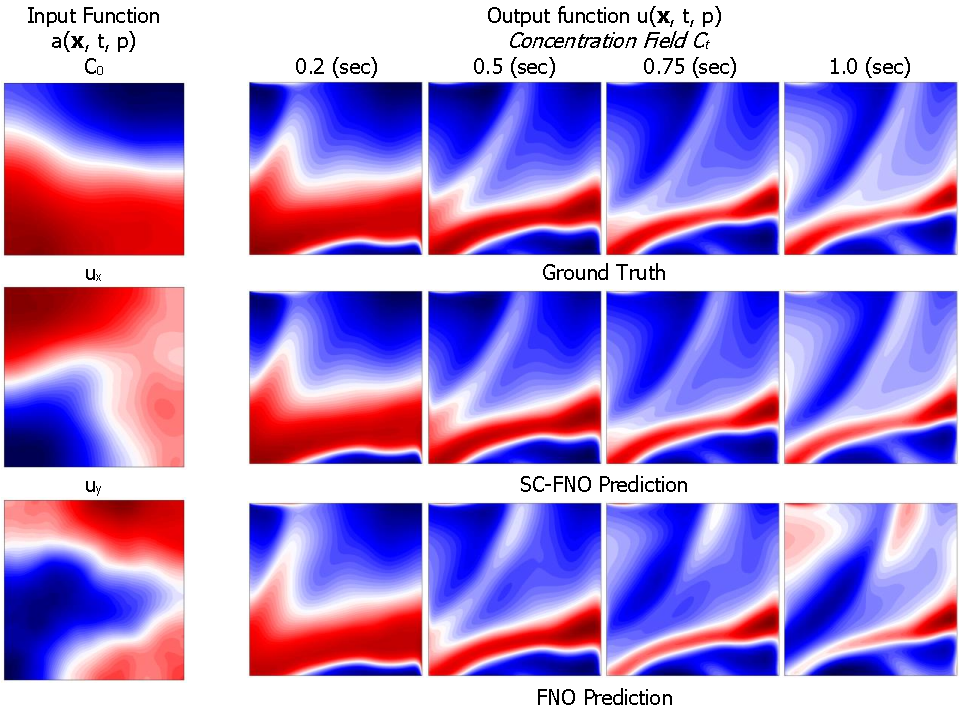
\includegraphics[width=0.8\textwidth, trim={0 0 0 0}, clip]{Figuers/PDE1_sample_prediction.pdf} % update filename if needed
%     \caption{\textbf{PDE1 Sample Prediction.}  
%     Representative forward prediction for PDE1 showing ground truth, SC-FNO, and FNO at selected time snapshots.  
%     SC-FNO remains closely aligned with the ground truth and avoids the dissipative errors observed in FNO.}
%     \label{fig:PDE1_sample_pred}
% \end{figure}




% Table for performances of models for inverse prediction of PDE1 without STD
\begin{table}[ht!]
\centering
\caption{\scriptsize\textbf{Comparison of Error Metrics Across Models Trained with Different Sample Sizes (Inverse)}}
\label{tab:pde1_inverse_nostd} 
\scriptsize
\setlength{\tabcolsep}{3pt}
\begin{tabular}{lcccccccc}
\hline
\textbf{Model} & \multicolumn{2}{c}{\textbf{1000 Samples}} & \multicolumn{2}{c}{\textbf{500 Samples}} & \multicolumn{2}{c}{\textbf{200 Samples}} & \multicolumn{2}{c}{\textbf{100 Samples}} \\
 & \textbf{Rel. \(L^2\)} & \textbf{MAE} & \textbf{Rel. \(L^2\)} & \textbf{MAE} & \textbf{Rel. \(L^2\)} & \textbf{MAE} & \textbf{Rel. \(L^2\)} & \textbf{MAE} \\
\hline
FNO & \(1.3 \times 10^{-1}\) & \(6.2 \times 10^{-2}\) & \(2.1 \times 10^{-1}\) & \(1.0 \times 10^{-1}\) & \(3.2 \times 10^{-1}\) & \(1.5 \times 10^{-1}\) & \(5.1 \times 10^{-1}\) & \(2.4 \times 10^{-1}\) \\
WNO & \(1.6 \times 10^{-1}\) & \(7.4 \times 10^{-2}\) & \(2.5 \times 10^{-1}\) & \(1.2 \times 10^{-1}\) & \(3.8 \times 10^{-1}\) & \(1.8 \times 10^{-1}\) & \(6.1 \times 10^{-1}\) & \(2.8 \times 10^{-1}\) \\
DeepONet & \(1.6 \times 10^{-1}\) & \(7.6 \times 10^{-2}\) & \(2.6 \times 10^{-1}\) & \(1.2 \times 10^{-1}\) & \(3.9 \times 10^{-1}\) & \(1.8 \times 10^{-1}\) & \(6.3 \times 10^{-1}\) & \(2.9 \times 10^{-1}\) \\
SC-FNO & \(\mathbf{1.3 \times 10^{-2}}\) & \(\mathbf{6.2 \times 10^{-3}}\) & \(\mathbf{1.5 \times 10^{-2}}\) & \(\mathbf{7.1 \times 10^{-3}}\) & \(\mathbf{1.8 \times 10^{-2}}\) & \(\mathbf{8.2 \times 10^{-3}}\) & \(\mathbf{2.1 \times 10^{-2}}\) & \(\mathbf{1.0 \times 10^{-2}}\) \\
SC-WNO & \(1.5 \times 10^{-2}\) & \(6.9 \times 10^{-3}\) & \(1.7 \times 10^{-2}\) & \(8.0 \times 10^{-3}\) & \(2.0 \times 10^{-2}\) & \(9.2 \times 10^{-3}\) & \(2.4 \times 10^{-2}\) & \(1.1 \times 10^{-2}\) \\
SC-DeepONet & \(1.8 \times 10^{-2}\) & \(8.4 \times 10^{-3}\) & \(2.1 \times 10^{-2}\) & \(9.7 \times 10^{-3}\) & \(2.4 \times 10^{-2}\) & \(1.1 \times 10^{-2}\) & \(2.9 \times 10^{-2}\) & \(1.4 \times 10^{-2}\) \\
\hline
\end{tabular}
\end{table}






% \begin{figure}[ht!]
%     \centering
%     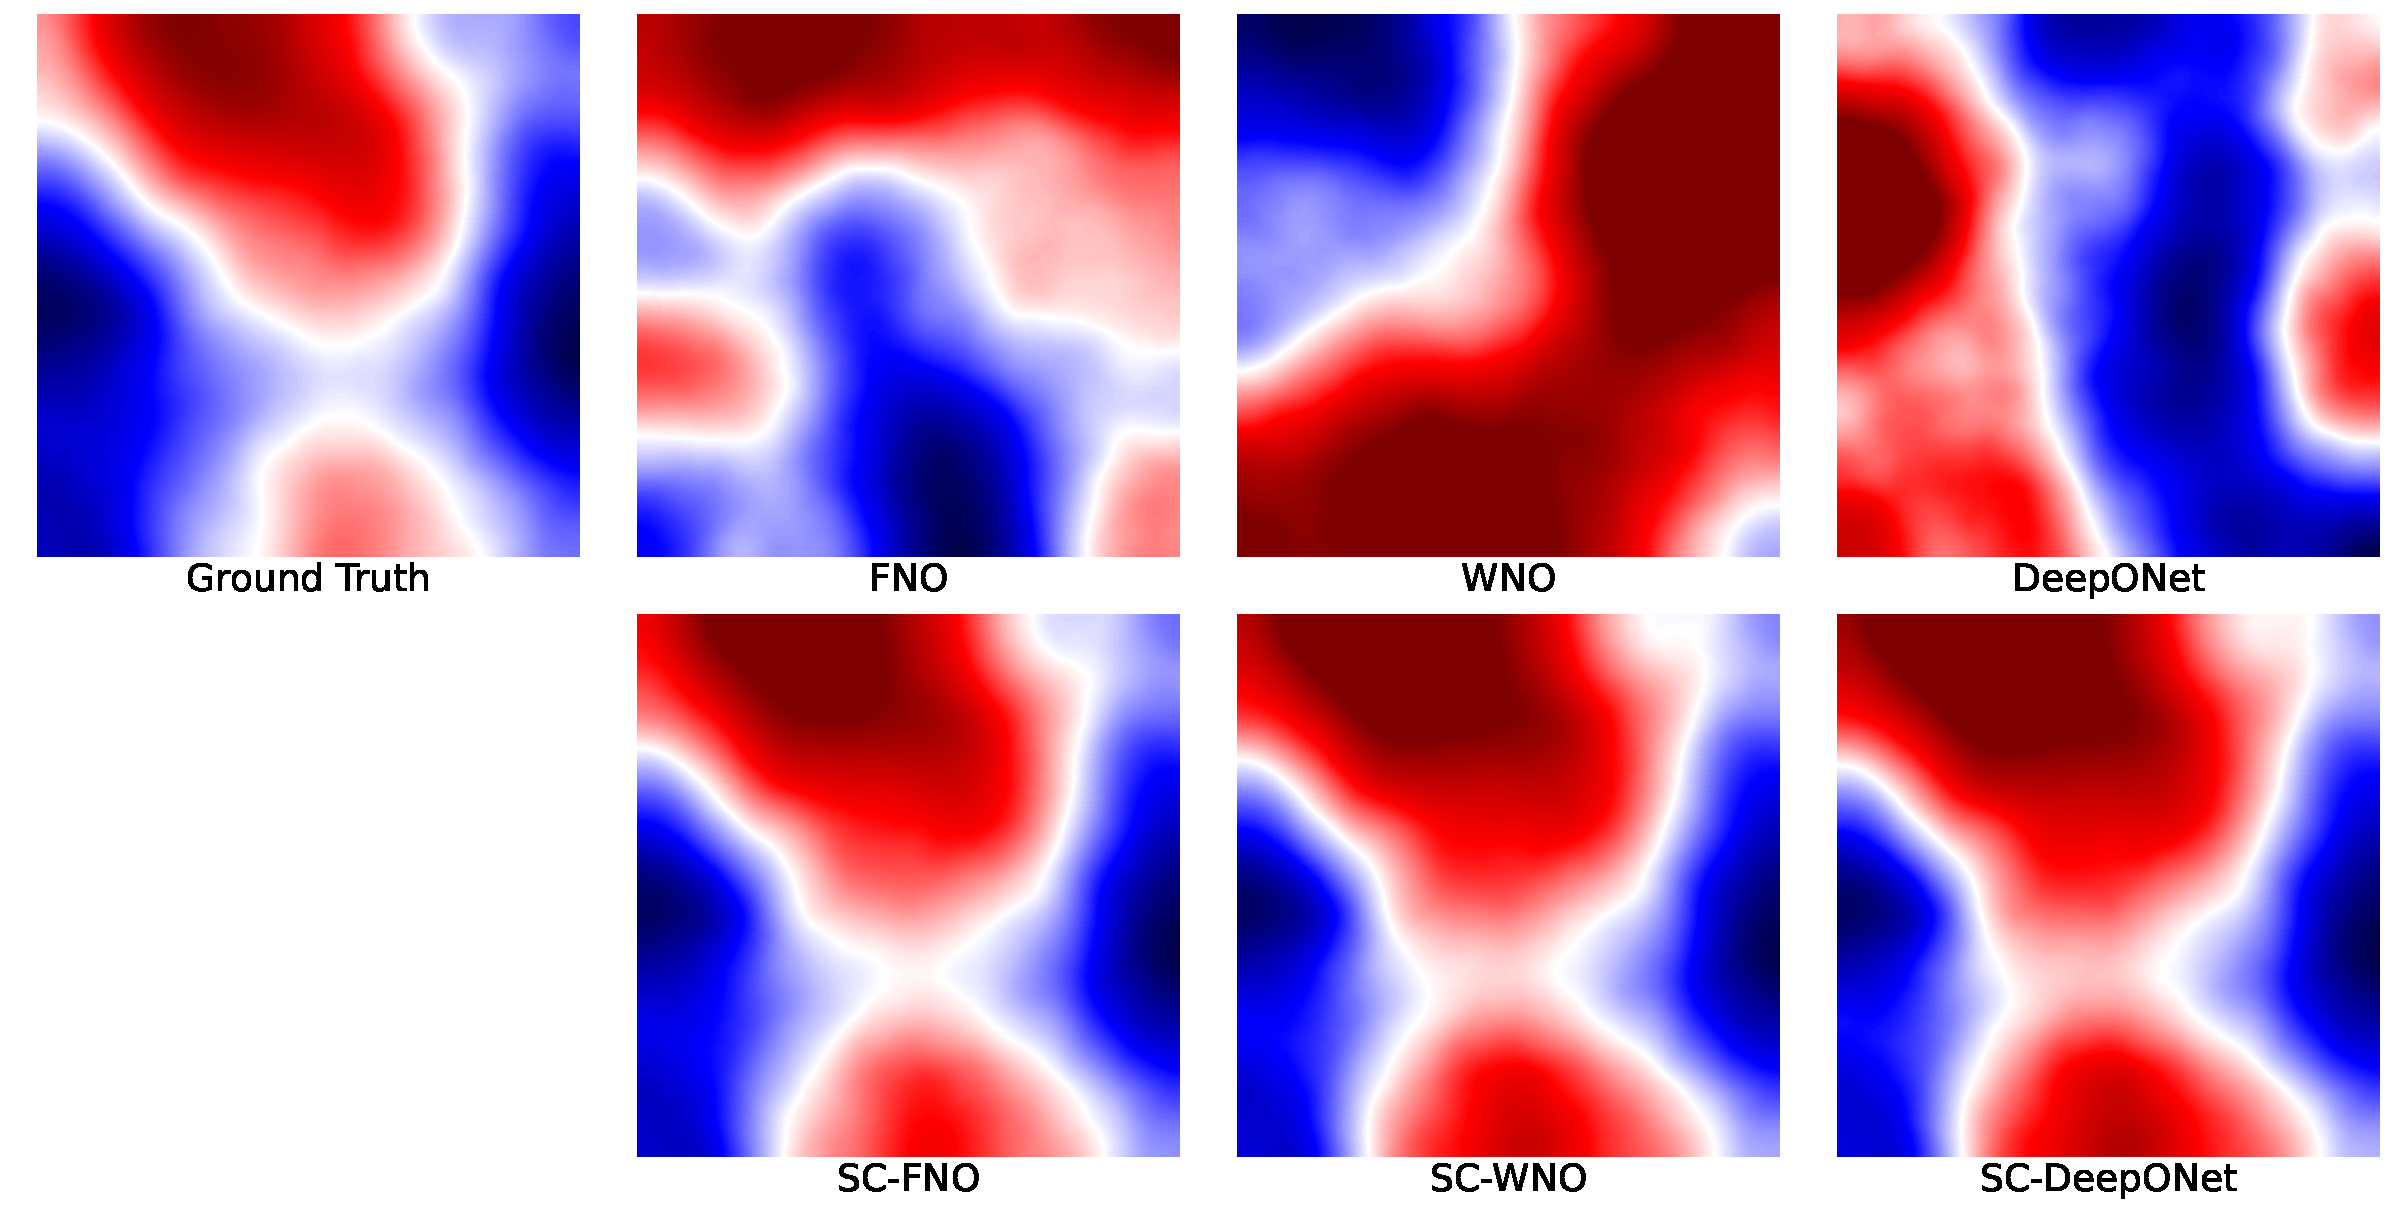
\includegraphics[width=0.8\textwidth]{Figuers/C0_ADE_reconstruction_clean_sample_10.pdf}
%     \caption{\textbf{Inversion of the initial concentration field for PDE1 (all models trained using 1000 samples).} 
%     Comparison of the true initial concentration field $C_0$ (top-left) with the inferred fields produced by FNO, WNO, DeepONet, and their sensitivity-constrained counterparts (SC-FNO, SC-WNO, SC-DeepONet).}    \label{fig:PDE1_C0_inversion}
%     \end{figure}


\begin{figure}[ht!]
    \centering
    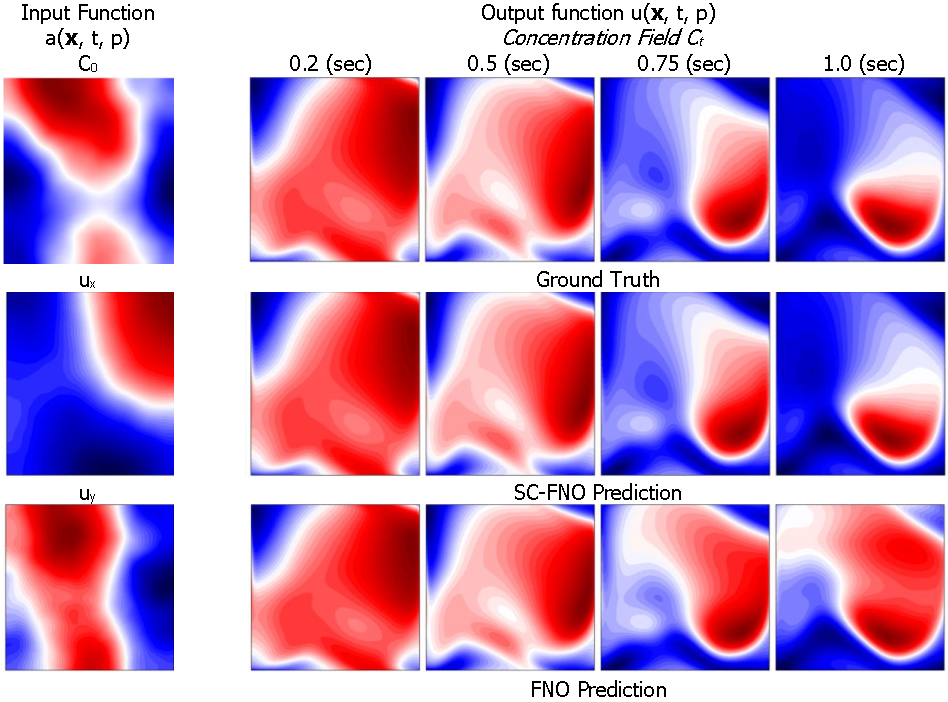
\includegraphics[width=0.8\textwidth, trim={0 0 0 0}, clip]{Figuers/PDE1_sample_prediction_1000_samples.pdf} % update filename if needed
    \caption{\scriptsize\textbf{PDE1 Sample Prediction.}  
    Representative forward prediction for PDE1 showing ground truth, SC-FNO, and FNO, trained on 1000 samples, at selected time snapshots.  
    SC-FNO remains closely aligned with the ground truth and avoids the dissipative errors observed in FNO.}
    \label{fig:PDE1_sample_pred}
\end{figure}






\begin{figure}[ht!]
    \centering
    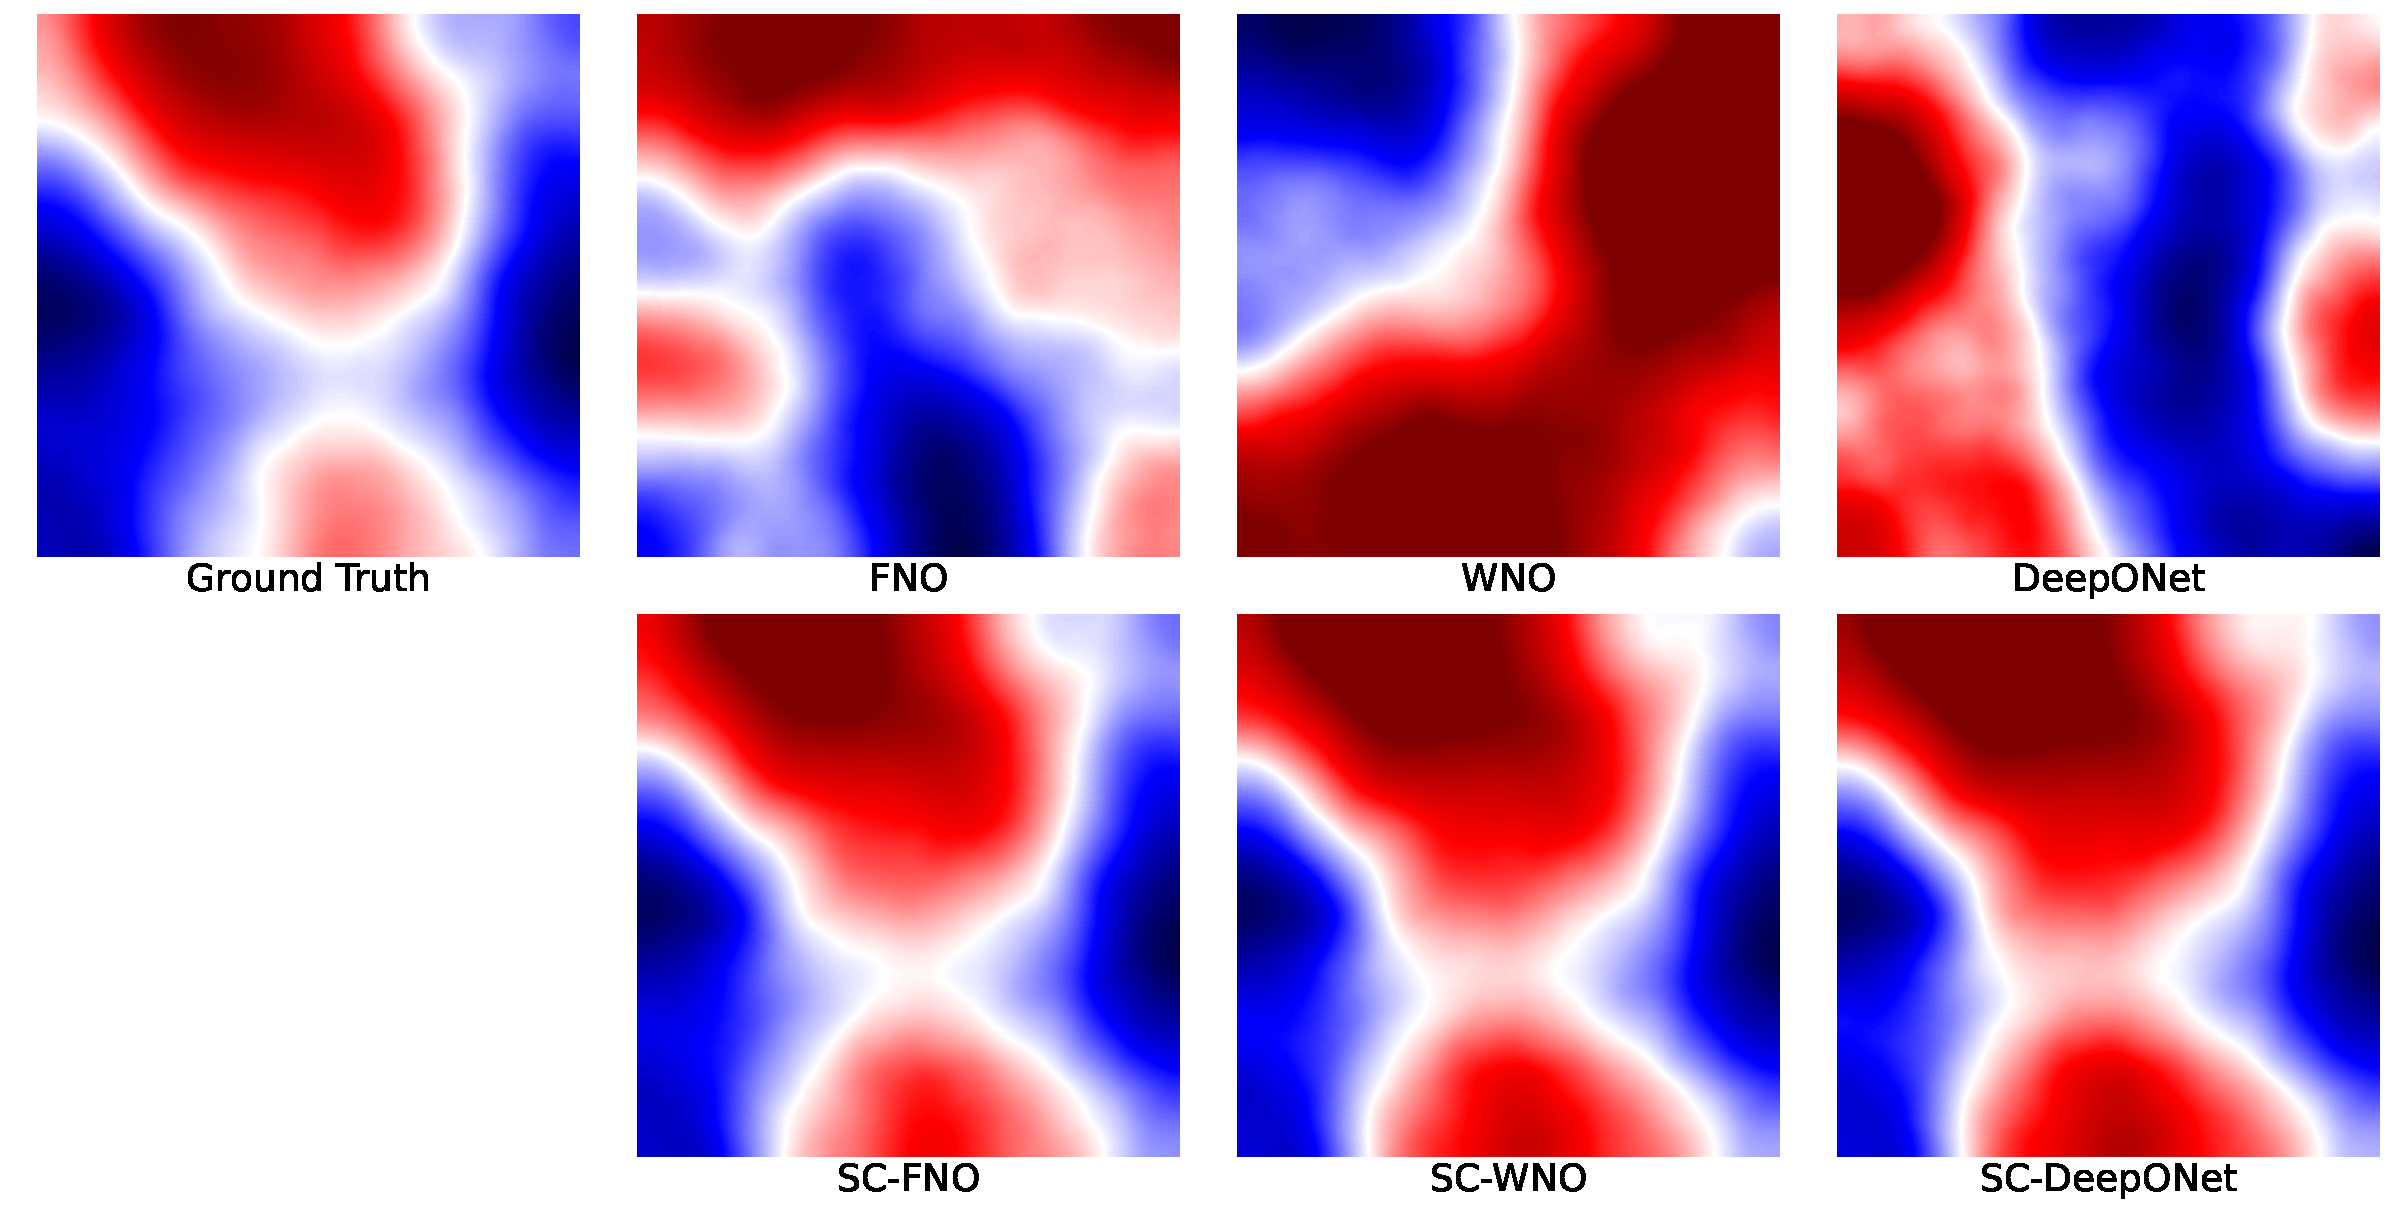
\includegraphics[width=0.8\textwidth]{Figuers/C0_ADE_reconstruction_clean_sample_10.pdf}
    \caption{\scriptsize\textbf{Inversion of the initial concentration field for PDE1 (all models trained using 200 samples).} 
    Comparison of the true initial concentration field $C_0$ (top-left) with the inferred fields produced by FNO, WNO, DeepONet, and their sensitivity-constrained counterparts (SC-FNO, SC-WNO, SC-DeepONet).}    \label{fig:PDE1_C0_inversion}
    \end{figure}

